% No Feedback on barriers
% Ying yang barriers & strategy

\section{Barriers towards an Open SDI}

With the current status of the SSDI clarified, we continue to the second part of the research question: "what are the challenges in the way of more openness". From the literature \& governmental publishing's analysed during the assessment, we distinguish three main barriers in place preventing the proper development of the SSDI: The uncertainties due to Brexit, a lack of public contribution, and a lack of cooperation among key stakeholders. 

\subsection{Brexit Uncertainties}

It is difficult to discuss the situation of the United Kingdom in general, or Scotland in particular, without mentioning Brexit. Regardless of the topic at hand, be it political, economical, social, or in our case the SDI, the withdrawal of the United Kingdom from the European Union has had a significant impact on all going-ons within the government of Scotland
\citep{impact_brexit}. In internal studies by the Scottish Government, it was concluded that civil servants describe Brexit as "working through the [...] fog of the fortnight ahead”. \citep{fog_of_brexit} . They state that their time-horizon has decreased to no further than two weeks, and this greatly troubles long term policy planning. This is a possible explanation for the fact that even though Scotland remains committed to the PSI directive, the progress of the SSDI has stagnated for the last four years \citep{impact_brexit}.

Since Brexit was finalized at the start of the current year, it is still uncertain how much of the shared geospatial data from across Europe is still freely and openly available to UK businesses, society and government \citep{impact_brexit}. Further investigation needs to be performed by British (and particularly Scottish) geospatial agencies in order to estimate the actual impact of this political decision for the geospatial sector in general.

\subsection{Lack of public contribution}

The Second major barrier is the barrier towards more participation, data participation in particular. 

Private individuals cannot create an account to contribute to the datasets \citep{ssdi_documentation}, as private individuals are not regarded by the SSDI as official users, only organizations are: "The portal does not currently allow self registration, and therefore interested parties should contact...". Currently, user accounts are created for organisations as a whole rather than individuals \citep{ssdi_documentation}. This means that private individuals should first become part of a certain group before they become a contributor of data. 



\subsection{Lack of Cooperation among stakeholders}

Finally, what we regard as the most major obstacle towards an SDI as described by the Open SDI theory stated in Van Loenen, 2018, is the lack of a clear all-encompassing vision towards precisely an Open SDI. This is prevented by the existence of multiple actors, with separate visions and mission statements covering only parts of the open SDI theory (Figure \ref{fig:actor-diagram}). 

\begin{figure}
    \hspace*{-4cm}
    \graphicspath{ {images/} }
    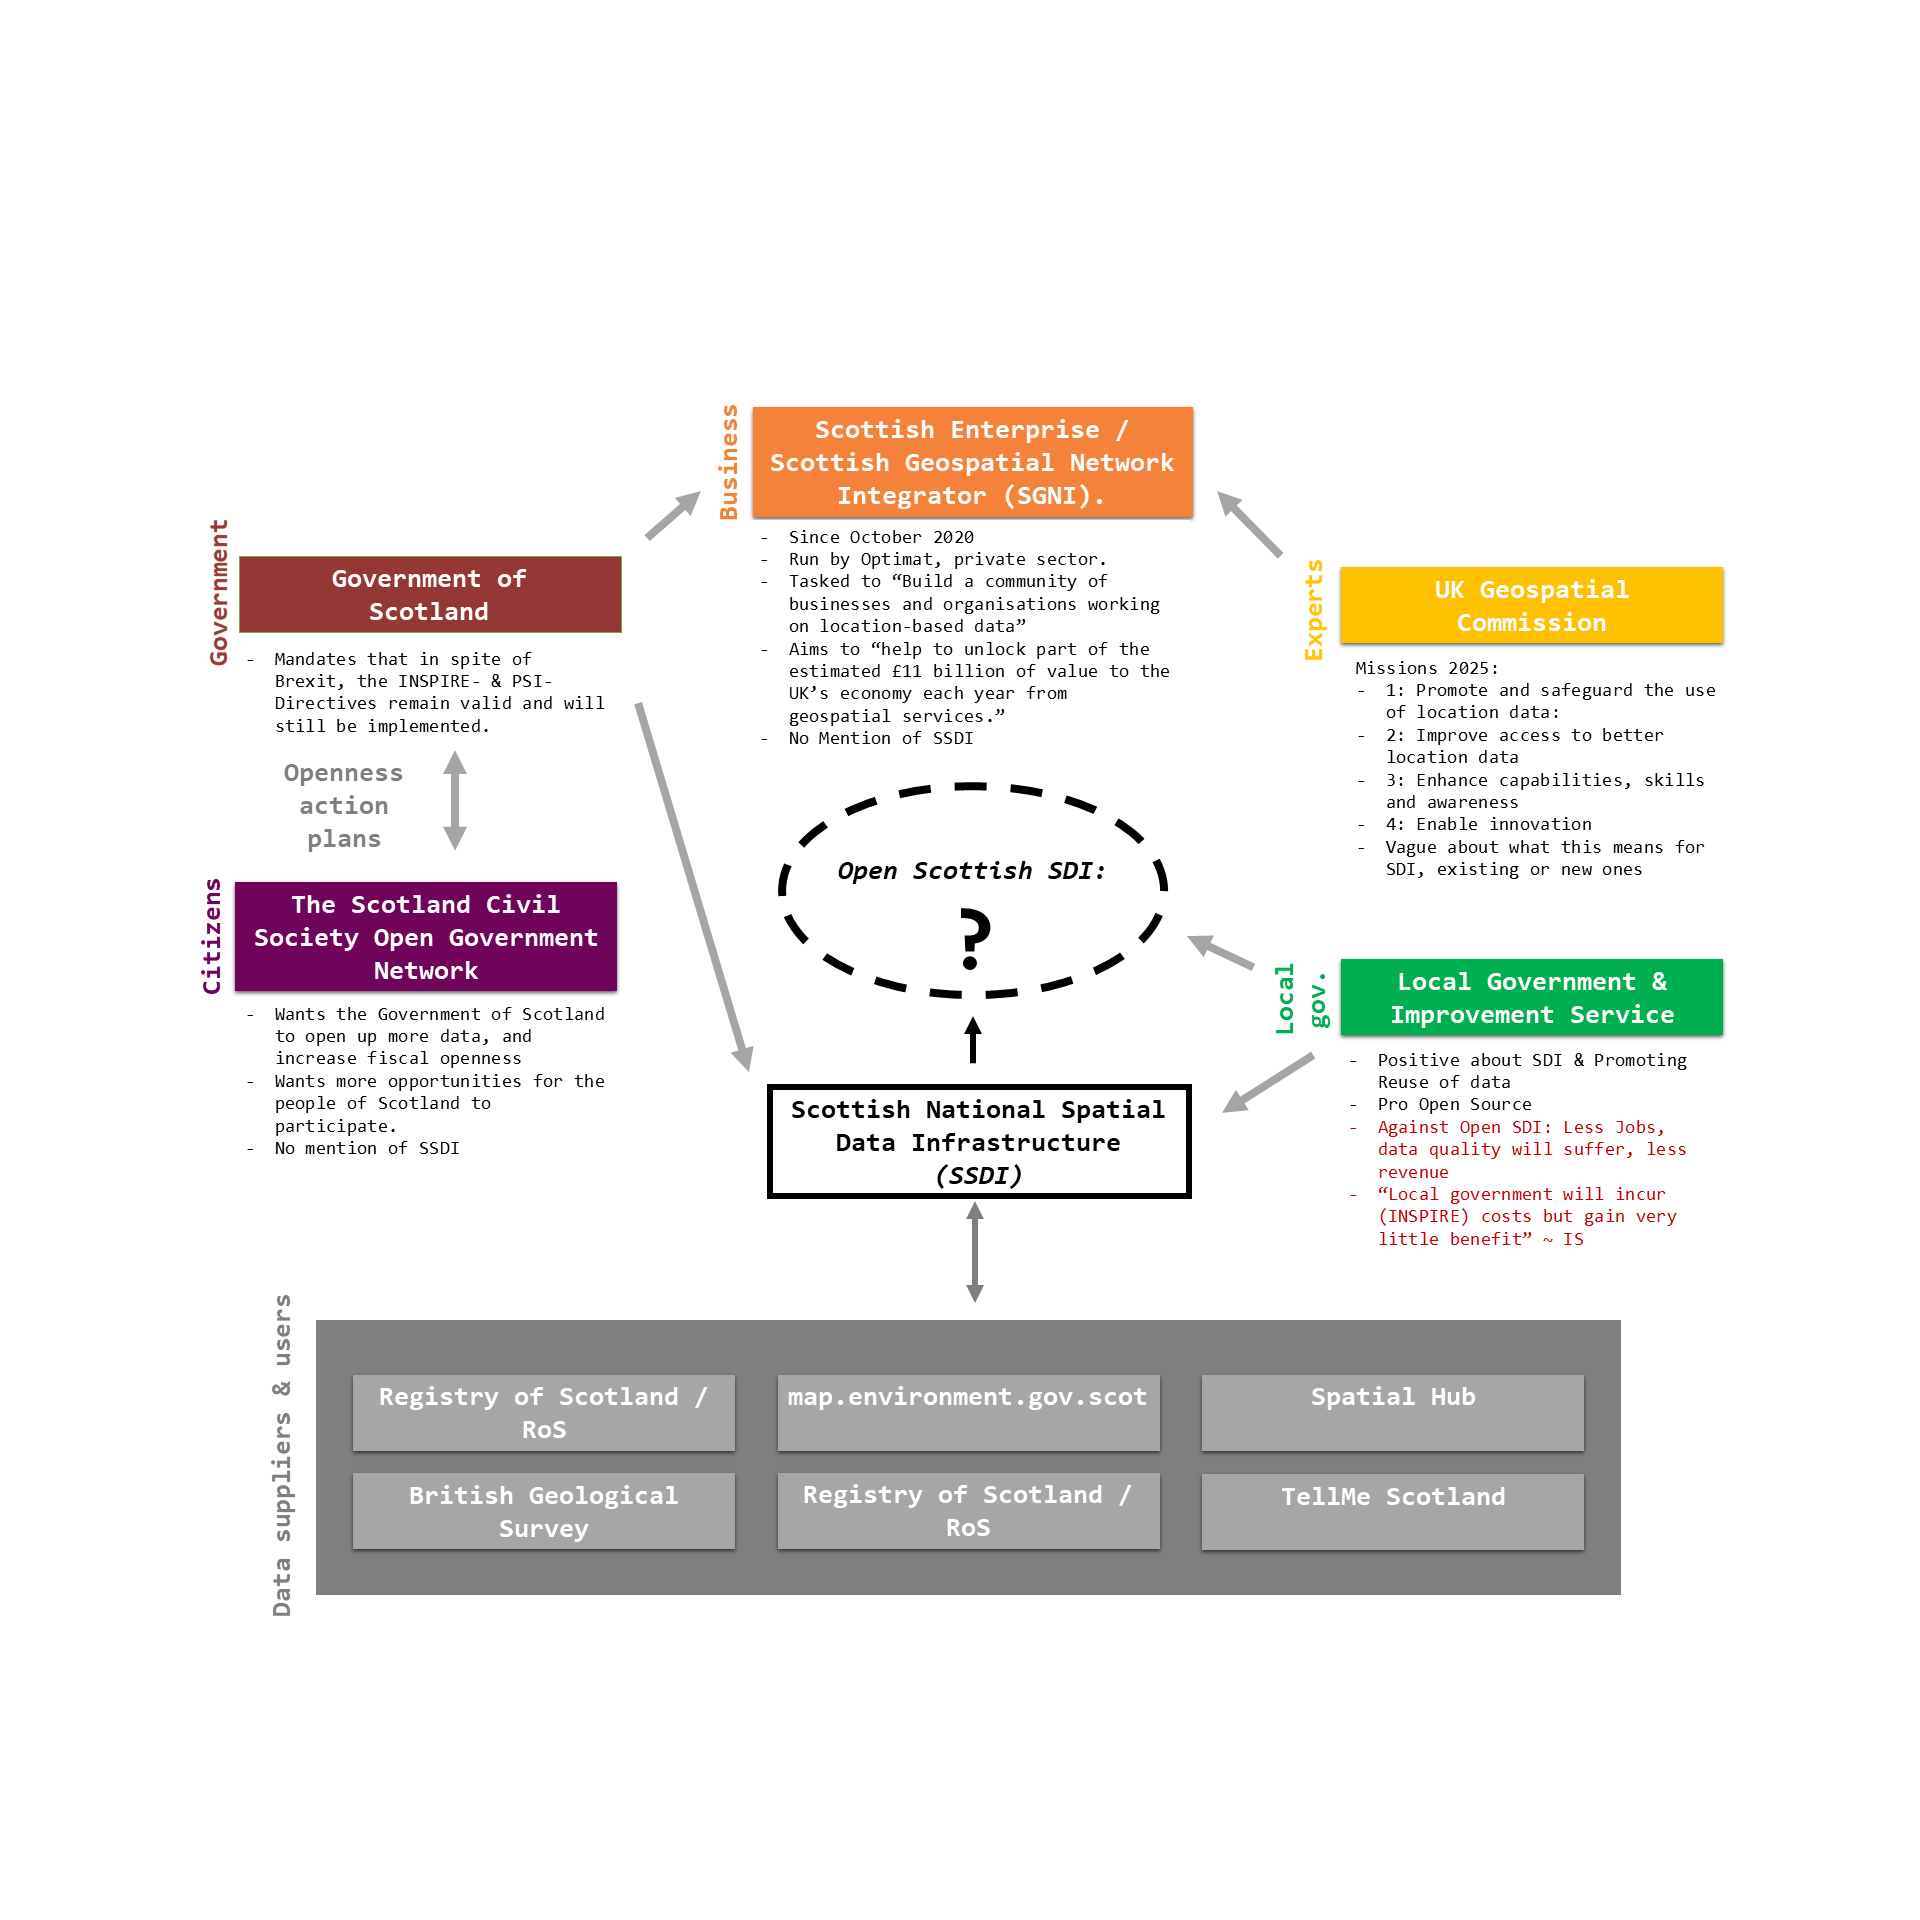
\includegraphics[width=22cm]{images/stakeholders.png}
    \caption{Actor Diagram. Sources: \citep{scottish_geospatial_network_integrator,impact_brexit, IS_local_SSDI, opengovpartnership_action_plan})}
    \label{fig:actor-diagram}
\end{figure}

This figure offers six main parties covering the needs of citizens, government, business, experts, local government, and the data providers \& users (produsers if you will). As shown, only a few of these actors mention the SSDI, and almost none of them refer to the idea of the Open SDI. Note also how the amount of active interactions \& collaborations (arrows) are limited. 

Plus, the fact that Figure \ref{fig:actor-diagram} couldn't be found and had to be made signals a clear lack of oversight on all parties involved. The Scottish Geospatial Network Integrator (in name of the Scottish Enterprise) has partly been created to mitigate this fragmentation \citep{scottish_geospatial_network_integrator}. "Scotland has a healthy geospatial sector but research by Scottish Enterprise has shown that more support is needed to encourage greater cooperation in the sector." \citep{scottish_geospatial_network_integrator}.